% !TeX root = ../main.tex
% Add the above to each chapter to make compiling the PDF easier in some editors.

\chapter{Introduction}\label{chapter:introduction}
Modern sensors, data infrastructures and traditional as well as machine learning algorithms have revolutionized the industry. As a key role in modern production facilities, Prognostic and Health Managment (PHM) applications have fully embraced the Big Data revolution. By analyzing production and machine data, future machine failures or working conditions can be predicted. This is especially helpful to prevent or at least warn employees about sudden and unexpected problems with production machines. The idea of PHM is to reduce the downtime of whole production lines \cite{ZHAO2019213}. Today's globalized world demands efficient internal processes and production strategies from companies. Therefore, the need for reliable PHM applications grew recently. Due to this increasing interest also the research focuses more and more on related topics. This thesis evaluates PHM approaches on a real production use case.

\section{Problems of Prognostics and Health Management for ball screw drives}
In a wide range of industrial machines, ball screws are used, which translate rotatory into linear motion with high precision. During longtime use, degradation lowers the stiffness within the ball screw components. This leads to an inaccurate position movement, which lowers the precision of the machine and therefore the production quality. In the worst case, a whole machine failure may occur. For this reason, tracking the ball screw health condition is of great importance. In recent years, PHM research mainly focused on rolling bearings and gearboxes. Since industrial machines and components have different operation conditions, working cycles and sensor installations, requirements for PHM algorithms vary. The transferability of PHM algorithms is limited and does usually require adjustments. However, intelligent data-driven methods have been successfully developed. Unfortunately, a lot of these approaches assume the training and testing data to be from the same data distribution. In reality, this is not the case. Since the operating conditions, component degradation and machine settings may change, the fault characteristics of the machines do also change. Fault diagnosis systems which are trained on a limited amount of data, which represents the machine fault characteristics partially, usually can't generalize well on the testing data with changed fault characteristics. Consequently, such diagnosis systems show unsatisfactory performance when being applied in real industrial scenarios over long periods of time. This phenomenon is called domain shift problem \cite{AZAMFAR2020103932}. In order to compensate the domain shift problem in health monitoring tasks, domain adaption and transfer learning approaches can be applied. These methods attempt to minimize the distribution discrepancy that occurs when recording machine data over a long period of time and is caused by the changed fault characteristics. 

\section{Traditional Prognostics and Health Management Approaches}
As shown in fig. \ref{fig:hand_crafted_features_physical_models_deep_learning} health monitoring is traditionally restricted to physical-based and conventional data-driven approaches. In the context of PHM, physical laws sound promising to explain the underlying complexity of a machine. These models are especially attractive since they don't require any historical fault data to make predictions about the health condition of a machine \cite{AN201942}. If the physics projected on the data doesn't include all relevant machine aspects as well as noise and perturbation, the performance of such approaches is reduced. With the upcoming modern sensors, networks and computing systems, data-driven approaches became more and more relevant for real world scenarios. In conventional data-driven approaches, traditional hand-crafted features are used to extract expressive information from the data in a first step. Subsequently, a shallow classifier predicts the corresponding health condition state for the samples. The just mentioned methods suffer from three problems. Firstly, in complex real-world scenarios, establishing physical-based models or conventional hand-crafted features is quite a laborious task and expects a lot of experience. Secondly, an on-line model update is not possible. Thirdly, the physical-based models and hand-crafted features are restricted to the application of interest and suffer from bad transferability. The limited flexibility and effectiveness of the two traditional approaches are responsible for the growing interest in deep learning based PHM. Deep neural networks can capture relations within complex and high-dimensional data. By using multiple layers, neural networks can progressively extract features with different levels of abstraction. The automatic learning makes neural networks easily adjustable to different problems. The popularity of neural networks exploded especially due to the increasing amount of data, computational power \cite{ZHAO2019213} \cite{AZAMFAR2020103932}. Especially, when using 

\begin{figure}[H]
  \centering
  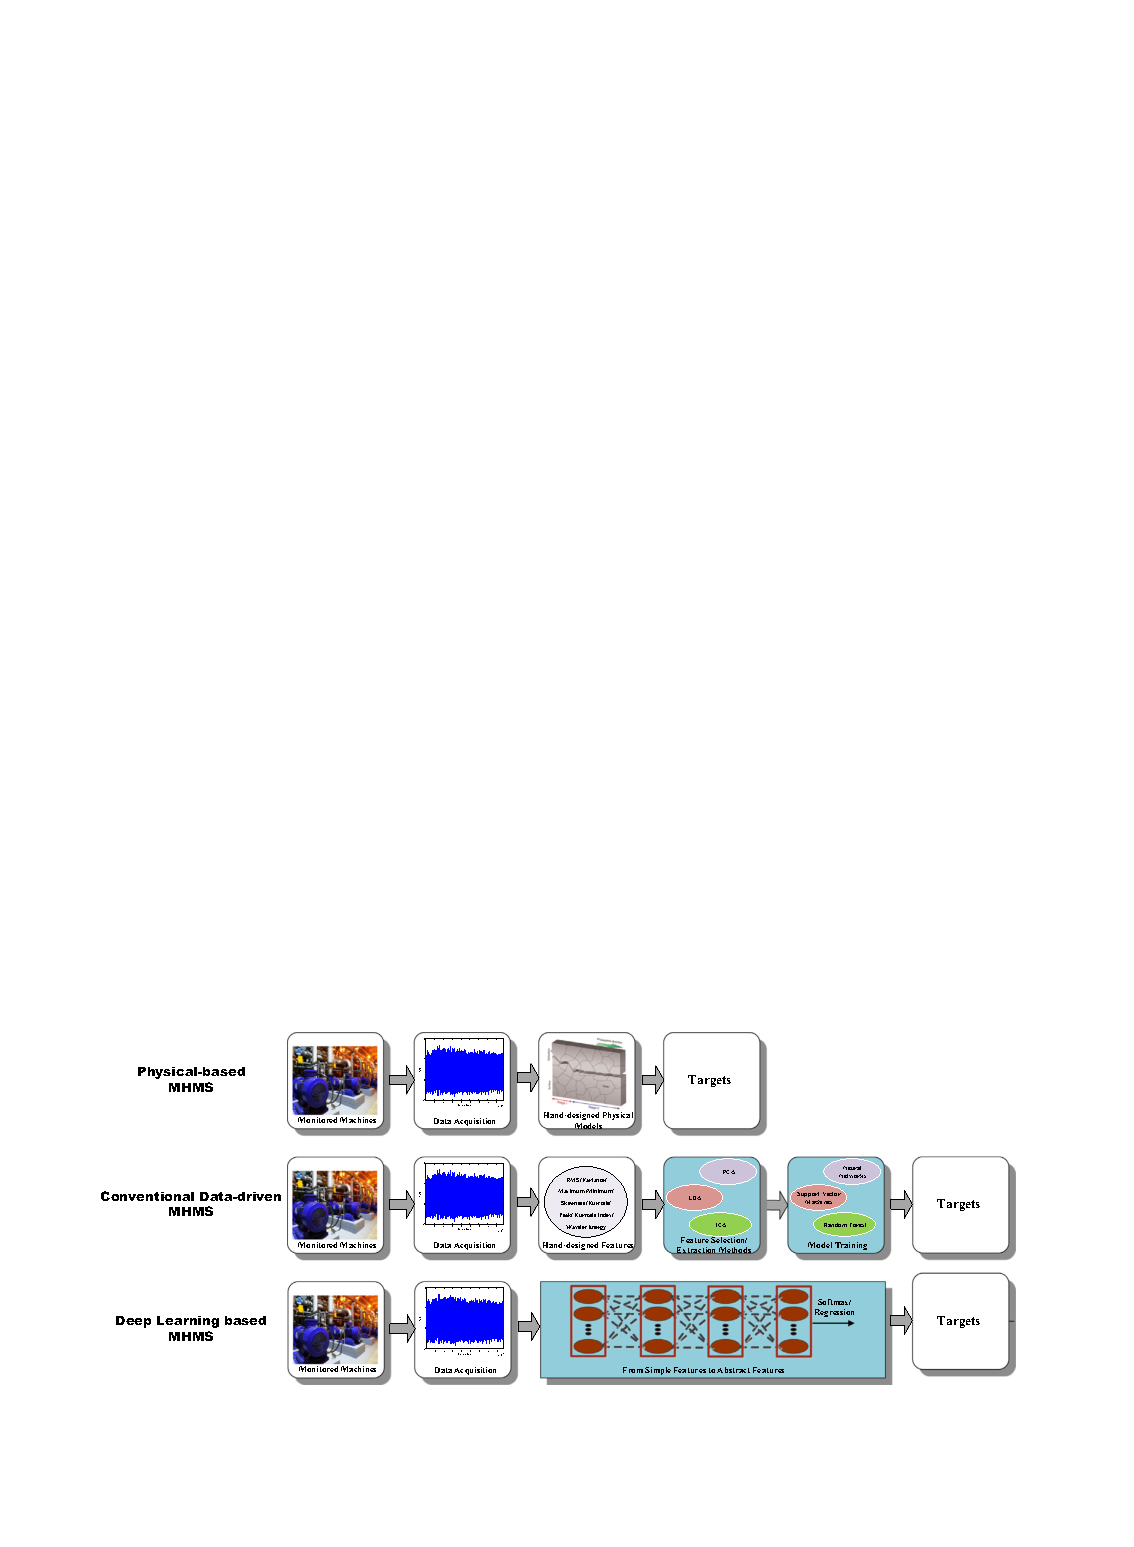
\includegraphics[width=1\textwidth]{hand_crafted_features_physical_models_deep_learning.pdf}
  \caption {Physical Models, Conventional Data-driven Models and Deep Learning Models for predictive maintenance \cite{ZHAO2019213}} \label{fig:hand_crafted_features_physical_models_deep_learning}
\end{figure}